\documentclass{beamer}
\usetheme{AnnArbor}
\usecolortheme{beaver}
\usepackage{graphicx}
\graphicspath{{images/}}
\usepackage[T1]{fontenc}
\usepackage[utf8x]{inputenc}
\usepackage[french]{babel}
\usepackage{subcaption}

\usepackage{mathtools} % Pour les symbols mathématiques

\title[Soutenance de fin d'études]{Automatisation de Test fonctionnel et de Test Non-régression}

\author{Qilin ZHANG}
\institute{Sorbonne Université - Master 2 Informatique STL Alternance}
\date{5 Septembre 2019}
\subject{presentation}

% Table des matières à chaque début de section
\AtBeginSection[]
{
  \begin{frame}
    \frametitle{Table of Contents}
    \tableofcontents[currentsection, currentsubsection]
  \end{frame}
}
\begin{document}
    % page de titre
    \begin{frame}
        \titlegraphic{
            
\includegraphics[width=2cm]{Logo_officiel_Sorbonne_University}\hspace*{1.75cm}~%
            
\includegraphics[width=2cm]{SAP_R_grad}
        }
        
        \titlepage
        \footnotesize Tuteur D'entreprise: Camilla CHRISTIANSEN, Sébastien COUDRAY \\
Tuteur universitaire: Emmanuel CHAILLOUX, Binh-Minh BUI-XUAN
    \end{frame}
    
    % Logo 
    \logo{
            
\includegraphics[height=0.5cm]{Logo_officiel_Sorbonne_University}
            
\includegraphics[height=0.5cm]{SAP_R_grad}
        }
        
    % plan
    \begin{frame}
        \frametitle{Plan}
        \tableofcontents
    \end{frame}
    
    \section{Présentation d'organisation d'accueil}
        \subsection{Présentation d'entreprise - SAP}
        
        %%%%%% Frame 1 %%%%%%
        \begin{frame}
            \begin{block} {SAP Histoire}
                SAP SE (Systeme, Anwendungen und Produkte in der Datenverarbeitung), fondé par 5 anciens IBM employés en 1972, 
                Concentrer aux clients d'entreprise
            \end{block}
            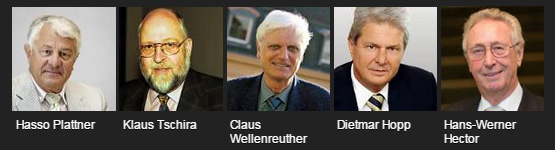
\includegraphics[width=7cm,]{sap_founders.jpg}
            
            
        \end{frame}
        
        %%%%%% Frame 2 %%%%%%
        \begin{frame}
            \begin{block}{SAP Produits}
                8 Catégories des produits en globales : 
                \begin{itemize}
                    \item ERP et coeur numérique
                    \item Gestion de la relation client et expérience client
                    \item Réseau et gestion des dépenses
                    \item Chaîne logistique digitale
                    \item RH et implication du personnel
                    \item Plateforme digitale
                    \item Outils d’analyse
                    \item Technologies intelligentes
                \end{itemize}
            \end{block}
            \pause
            \begin{block}{Le produit que je travaille sur}
            \textbf{SAP Financial Consolidation}, la catégorie ERP et coeur numérique
            \end{block}
        \end{frame}
        
        %%%%%% Frame 3 %%%%%%
        \begin{frame}
            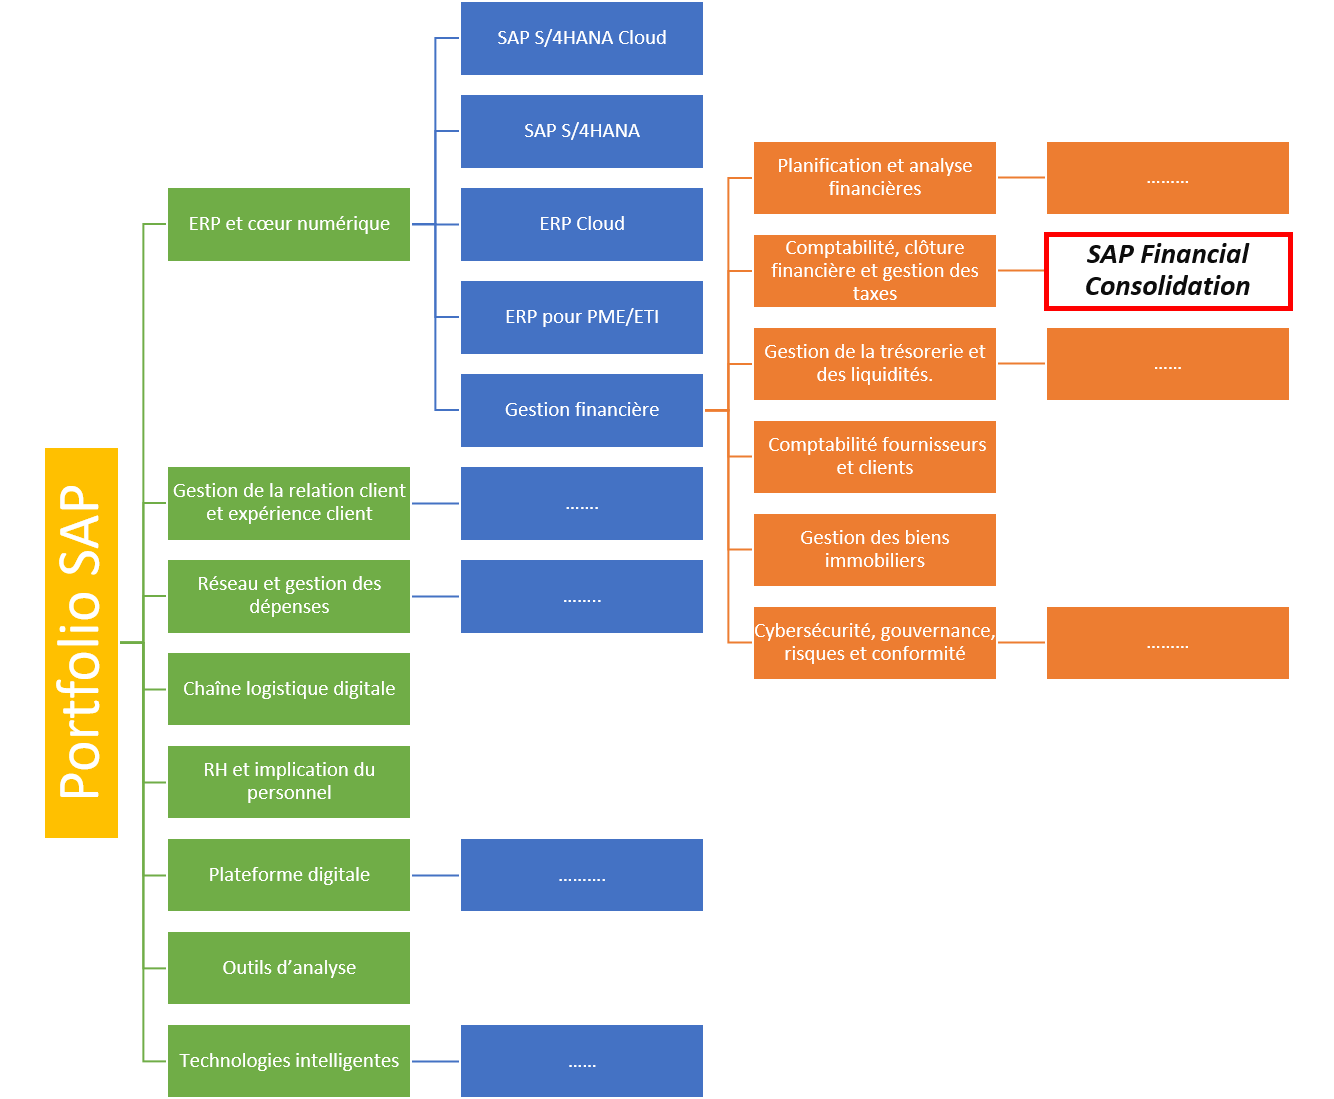
\includegraphics[height=8cm]{SAP_portfolio.png}
        \end{frame}
        
        \subsection{Introduction d'équipe}
        %%%%%% Frame 4 %%%%%%
        \begin{frame}
        \frametitle{Organisation d'équipe et mon rôle}
            
        \end{frame}
        
        
    \section{Contexte et la problématique}
        
        \subsection{Produit SAP Financial Consolidation}
        %%%%%% Frame 5 %%%%%%
        \begin{frame}
        \frametitle{Frame Title}
            
        \end{frame}
        
        \subsection{Test régression et Test non-régression}
        \begin{frame}
        \frametitle{Frame Title}
            
        \end{frame}
        
        \subsection{Test d'impression}
        \begin{frame}
        \frametitle{Frame Title}
            
        \end{frame}
        
    \section{Travaux Réalisés}
        \subsection{Architecture de Test auto}
        \begin{frame}
        \frametitle{frametitle}    
        \end{frame}
        
        \subsection{Cycle de vie de Test d'impression}
        \begin{frame}
        \frametitle{Frame Title}
            
        \end{frame}
        
        \subsection{Développements Réalisés}
        \begin{frame}
        \frametitle{Comparaison entre deux PDF}
            
        \end{frame}
        
        \begin{frame}
        \frametitle{Téléchargement de zip et unzip}
            
        \end{frame}
        
        \begin{frame}
        \frametitle{Comparaison entre deux répertoire avec $\lambda$}
            
        \end{frame}
        
    \section{Conclusion}
        \begin{frame}
        \frametitle{frametitle}
        \end{frame}
        
        \begin{frame}
            \begin{center}
                \Large{Merci pour votre attention !}
            \end{center}
            
        \end{frame}
\end{document}